% Options for packages loaded elsewhere
% Options for packages loaded elsewhere
\PassOptionsToPackage{unicode}{hyperref}
\PassOptionsToPackage{hyphens}{url}
%
\documentclass[
  ignorenonframetext,
]{beamer}
\newif\ifbibliography
\usepackage{pgfpages}
\setbeamertemplate{caption}[numbered]
\setbeamertemplate{caption label separator}{: }
\setbeamercolor{caption name}{fg=normal text.fg}
\beamertemplatenavigationsymbolsempty
% remove section numbering
\setbeamertemplate{part page}{
  \centering
  \begin{beamercolorbox}[sep=16pt,center]{part title}
    \usebeamerfont{part title}\insertpart\par
  \end{beamercolorbox}
}
\setbeamertemplate{section page}{
  \centering
  \begin{beamercolorbox}[sep=12pt,center]{section title}
    \usebeamerfont{section title}\insertsection\par
  \end{beamercolorbox}
}
\setbeamertemplate{subsection page}{
  \centering
  \begin{beamercolorbox}[sep=8pt,center]{subsection title}
    \usebeamerfont{subsection title}\insertsubsection\par
  \end{beamercolorbox}
}
% Prevent slide breaks in the middle of a paragraph
\widowpenalties 1 10000
\raggedbottom
\AtBeginPart{
  \frame{\partpage}
}
\AtBeginSection{
  \ifbibliography
  \else
    \frame{\sectionpage}
  \fi
}
\AtBeginSubsection{
  \frame{\subsectionpage}
}
\usepackage{iftex}
\ifPDFTeX
  \usepackage[T1]{fontenc}
  \usepackage[utf8]{inputenc}
  \usepackage{textcomp} % provide euro and other symbols
\else % if luatex or xetex
  \usepackage{unicode-math} % this also loads fontspec
  \defaultfontfeatures{Scale=MatchLowercase}
  \defaultfontfeatures[\rmfamily]{Ligatures=TeX,Scale=1}
\fi
\usepackage{lmodern}

\usetheme[]{CambridgeUS}
\usecolortheme[]{rose}
\usefonttheme[]{professionalfonts}
\ifPDFTeX\else
  % xetex/luatex font selection
\fi
% Use upquote if available, for straight quotes in verbatim environments
\IfFileExists{upquote.sty}{\usepackage{upquote}}{}
\IfFileExists{microtype.sty}{% use microtype if available
  \usepackage[]{microtype}
  \UseMicrotypeSet[protrusion]{basicmath} % disable protrusion for tt fonts
}{}
\makeatletter
\@ifundefined{KOMAClassName}{% if non-KOMA class
  \IfFileExists{parskip.sty}{%
    \usepackage{parskip}
  }{% else
    \setlength{\parindent}{0pt}
    \setlength{\parskip}{6pt plus 2pt minus 1pt}}
}{% if KOMA class
  \KOMAoptions{parskip=half}}
\makeatother

\usepackage{color}
\usepackage{fancyvrb}
\newcommand{\VerbBar}{|}
\newcommand{\VERB}{\Verb[commandchars=\\\{\}]}
\DefineVerbatimEnvironment{Highlighting}{Verbatim}{commandchars=\\\{\}}
% Add ',fontsize=\small' for more characters per line
\usepackage{framed}
\definecolor{shadecolor}{RGB}{241,243,245}
\newenvironment{Shaded}{\begin{snugshade}}{\end{snugshade}}
\newcommand{\AlertTok}[1]{\textcolor[rgb]{0.68,0.00,0.00}{#1}}
\newcommand{\AnnotationTok}[1]{\textcolor[rgb]{0.37,0.37,0.37}{#1}}
\newcommand{\AttributeTok}[1]{\textcolor[rgb]{0.40,0.45,0.13}{#1}}
\newcommand{\BaseNTok}[1]{\textcolor[rgb]{0.68,0.00,0.00}{#1}}
\newcommand{\BuiltInTok}[1]{\textcolor[rgb]{0.00,0.23,0.31}{#1}}
\newcommand{\CharTok}[1]{\textcolor[rgb]{0.13,0.47,0.30}{#1}}
\newcommand{\CommentTok}[1]{\textcolor[rgb]{0.37,0.37,0.37}{#1}}
\newcommand{\CommentVarTok}[1]{\textcolor[rgb]{0.37,0.37,0.37}{\textit{#1}}}
\newcommand{\ConstantTok}[1]{\textcolor[rgb]{0.56,0.35,0.01}{#1}}
\newcommand{\ControlFlowTok}[1]{\textcolor[rgb]{0.00,0.23,0.31}{\textbf{#1}}}
\newcommand{\DataTypeTok}[1]{\textcolor[rgb]{0.68,0.00,0.00}{#1}}
\newcommand{\DecValTok}[1]{\textcolor[rgb]{0.68,0.00,0.00}{#1}}
\newcommand{\DocumentationTok}[1]{\textcolor[rgb]{0.37,0.37,0.37}{\textit{#1}}}
\newcommand{\ErrorTok}[1]{\textcolor[rgb]{0.68,0.00,0.00}{#1}}
\newcommand{\ExtensionTok}[1]{\textcolor[rgb]{0.00,0.23,0.31}{#1}}
\newcommand{\FloatTok}[1]{\textcolor[rgb]{0.68,0.00,0.00}{#1}}
\newcommand{\FunctionTok}[1]{\textcolor[rgb]{0.28,0.35,0.67}{#1}}
\newcommand{\ImportTok}[1]{\textcolor[rgb]{0.00,0.46,0.62}{#1}}
\newcommand{\InformationTok}[1]{\textcolor[rgb]{0.37,0.37,0.37}{#1}}
\newcommand{\KeywordTok}[1]{\textcolor[rgb]{0.00,0.23,0.31}{\textbf{#1}}}
\newcommand{\NormalTok}[1]{\textcolor[rgb]{0.00,0.23,0.31}{#1}}
\newcommand{\OperatorTok}[1]{\textcolor[rgb]{0.37,0.37,0.37}{#1}}
\newcommand{\OtherTok}[1]{\textcolor[rgb]{0.00,0.23,0.31}{#1}}
\newcommand{\PreprocessorTok}[1]{\textcolor[rgb]{0.68,0.00,0.00}{#1}}
\newcommand{\RegionMarkerTok}[1]{\textcolor[rgb]{0.00,0.23,0.31}{#1}}
\newcommand{\SpecialCharTok}[1]{\textcolor[rgb]{0.37,0.37,0.37}{#1}}
\newcommand{\SpecialStringTok}[1]{\textcolor[rgb]{0.13,0.47,0.30}{#1}}
\newcommand{\StringTok}[1]{\textcolor[rgb]{0.13,0.47,0.30}{#1}}
\newcommand{\VariableTok}[1]{\textcolor[rgb]{0.07,0.07,0.07}{#1}}
\newcommand{\VerbatimStringTok}[1]{\textcolor[rgb]{0.13,0.47,0.30}{#1}}
\newcommand{\WarningTok}[1]{\textcolor[rgb]{0.37,0.37,0.37}{\textit{#1}}}

\usepackage{longtable,booktabs,array}
\usepackage{calc} % for calculating minipage widths
\usepackage{caption}
% Make caption package work with longtable
\makeatletter
\def\fnum@table{\tablename~\thetable}
\makeatother
\usepackage{graphicx}
\makeatletter
\newsavebox\pandoc@box
\newcommand*\pandocbounded[1]{% scales image to fit in text height/width
  \sbox\pandoc@box{#1}%
  \Gscale@div\@tempa{\textheight}{\dimexpr\ht\pandoc@box+\dp\pandoc@box\relax}%
  \Gscale@div\@tempb{\linewidth}{\wd\pandoc@box}%
  \ifdim\@tempb\p@<\@tempa\p@\let\@tempa\@tempb\fi% select the smaller of both
  \ifdim\@tempa\p@<\p@\scalebox{\@tempa}{\usebox\pandoc@box}%
  \else\usebox{\pandoc@box}%
  \fi%
}
% Set default figure placement to htbp
\def\fps@figure{htbp}
\makeatother





\setlength{\emergencystretch}{3em} % prevent overfull lines

\providecommand{\tightlist}{%
  \setlength{\itemsep}{0pt}\setlength{\parskip}{0pt}}



 


\makeatletter
\@ifpackageloaded{tcolorbox}{}{\usepackage[skins,breakable]{tcolorbox}}
\@ifpackageloaded{fontawesome5}{}{\usepackage{fontawesome5}}
\definecolor{quarto-callout-color}{HTML}{909090}
\definecolor{quarto-callout-note-color}{HTML}{0758E5}
\definecolor{quarto-callout-important-color}{HTML}{CC1914}
\definecolor{quarto-callout-warning-color}{HTML}{EB9113}
\definecolor{quarto-callout-tip-color}{HTML}{00A047}
\definecolor{quarto-callout-caution-color}{HTML}{FC5300}
\definecolor{quarto-callout-color-frame}{HTML}{acacac}
\definecolor{quarto-callout-note-color-frame}{HTML}{4582ec}
\definecolor{quarto-callout-important-color-frame}{HTML}{d9534f}
\definecolor{quarto-callout-warning-color-frame}{HTML}{f0ad4e}
\definecolor{quarto-callout-tip-color-frame}{HTML}{02b875}
\definecolor{quarto-callout-caution-color-frame}{HTML}{fd7e14}
\makeatother
\makeatletter
\@ifpackageloaded{caption}{}{\usepackage{caption}}
\AtBeginDocument{%
\ifdefined\contentsname
  \renewcommand*\contentsname{Table of contents}
\else
  \newcommand\contentsname{Table of contents}
\fi
\ifdefined\listfigurename
  \renewcommand*\listfigurename{List of Figures}
\else
  \newcommand\listfigurename{List of Figures}
\fi
\ifdefined\listtablename
  \renewcommand*\listtablename{List of Tables}
\else
  \newcommand\listtablename{List of Tables}
\fi
\ifdefined\figurename
  \renewcommand*\figurename{Figure}
\else
  \newcommand\figurename{Figure}
\fi
\ifdefined\tablename
  \renewcommand*\tablename{Table}
\else
  \newcommand\tablename{Table}
\fi
}
\@ifpackageloaded{float}{}{\usepackage{float}}
\floatstyle{ruled}
\@ifundefined{c@chapter}{\newfloat{codelisting}{h}{lop}}{\newfloat{codelisting}{h}{lop}[chapter]}
\floatname{codelisting}{Listing}
\newcommand*\listoflistings{\listof{codelisting}{List of Listings}}
\makeatother
\makeatletter
\makeatother
\makeatletter
\@ifpackageloaded{caption}{}{\usepackage{caption}}
\@ifpackageloaded{subcaption}{}{\usepackage{subcaption}}
\makeatother

\usepackage{bookmark}
\IfFileExists{xurl.sty}{\usepackage{xurl}}{} % add URL line breaks if available
\urlstyle{same}
\hypersetup{
  pdftitle={Descubriendo Patrones con Frecuencias Simples},
  pdfauthor={Mario Morales},
  hidelinks,
  pdfcreator={LaTeX via pandoc}}


\title{Descubriendo Patrones con Frecuencias Simples}
\subtitle{Con datos de ejemplos de R}
\author{Mario Morales}
\date{01/03/2026}

\begin{document}
\frame{\titlepage}

\renewcommand*\contentsname{Table of contents}
\begin{frame}[allowframebreaks]
  \frametitle{Table of contents}
  \setcounter{tocdepth}{3}
  \tableofcontents
\end{frame}
\setcounter{tocdepth}{3}
\tableofcontents
}

\section{Fecha de entrega: Escriba aquí la fecha en formato
DD/MM/YYYY}\label{fecha-de-entrega-escriba-aquuxed-la-fecha-en-formato-ddmmyyyy}

\begin{frame}[fragile]{1. Introducción}
\phantomsection\label{introducciuxf3n}
En este taller aplicaremos los conceptos de \textbf{Distribuciones de
Frecuencia Simples} vistos en clase . Utilizaremos el conjunto de datos
\texttt{mtcars} para analizar variables discretas.

(lúscase aquí con una buena introducción, hable de lo que va a hacer y
como lo va a hacer)
\end{frame}

\begin{frame}[fragile]{2. Carga de Datos y Preparación}
\phantomsection\label{carga-de-datos-y-preparaciuxf3n}
Primero, cargaremos los datos y seleccionaremos la variable
\texttt{gear} (número de marchas).
\end{frame}

\begin{frame}{3. Continúe usted}
\phantomsection\label{continuxfae-usted}
\begin{tcolorbox}[enhanced jigsaw, opacitybacktitle=0.6, toprule=.15mm, opacityback=0, colbacktitle=quarto-callout-caution-color!10!white, colback=white, leftrule=.75mm, bottomrule=.15mm, colframe=quarto-callout-caution-color-frame, titlerule=0mm, coltitle=black, bottomtitle=1mm, breakable, rightrule=.15mm, toptitle=1mm, title=\textcolor{quarto-callout-caution-color}{\faFire}\hspace{0.5em}{Caution}, arc=.35mm, left=2mm]

\begin{itemize}
\item
  Para los gráficos use un color específico basado en la última letra de
  su nombre, de la siguiente forma.

  \begin{itemize}
  \tightlist
  \item
    Si su nombre inicia con la letra a, b, c, d, e, f entonces use el
    color {seagreen}
  \item
    Si su nombre inicia con la letra g, h, i, j, k, l, m entonces use el
    color {indianred}\\
  \item
    Si su nombre inicia con la letra n, o, p, q, r, s, t entonces use el
    color {steelblue}
  \item
    Si su nombre inicia con la letra u, v, w, x, y, z entonces use el
    color {darkorange}
  \end{itemize}
\end{itemize}

\end{tcolorbox}
\end{frame}

\begin{frame}{Mucho cuidado con estas reglas de juego.}
\phantomsection\label{mucho-cuidado-con-estas-reglas-de-juego.}
\begin{tcolorbox}[enhanced jigsaw, opacitybacktitle=0.6, toprule=.15mm, opacityback=0, colbacktitle=quarto-callout-caution-color!10!white, colback=white, leftrule=.75mm, bottomrule=.15mm, colframe=quarto-callout-caution-color-frame, titlerule=0mm, coltitle=black, bottomtitle=1mm, breakable, rightrule=.15mm, toptitle=1mm, title=\textcolor{quarto-callout-caution-color}{\faFire}\hspace{0.5em}{Caution}, arc=.35mm, left=2mm]

\begin{itemize}
\item
  Ojo con copias, con abuzar de la IA, quiero comentarios suyos sobre
  los resultados, no quiero solo código, lo importante es concluir a
  partir del resultado del código.
\item
  Pasaré los trabajos por la IA para que descubra dos cosas

  \begin{itemize}
  \tightlist
  \item
    Trabajos hechos por una IA
  \item
    Trabajos coincidentes, por ejemplo aquellos que piden el fuente y
    luego cambian el nombre y compilan, tendrán una fuerte penalización
    sin importar de quien es el original.
  \end{itemize}
\end{itemize}

\end{tcolorbox}
\end{frame}

\begin{frame}[fragile]{Visualización Gráfica}
\phantomsection\label{visualizaciuxf3n-gruxe1fica}
\begin{block}{Ejemplo de cómo deben aplicar el color:}
\phantomsection\label{ejemplo-de-cuxf3mo-deben-aplicar-el-color}
\begin{Shaded}
\begin{Highlighting}[]
\FunctionTok{barplot}\NormalTok{(ni, }
        \AttributeTok{main =} \StringTok{"Distribución de Frecuencias"}\NormalTok{,}
        \AttributeTok{xlab =} \StringTok{"Variable de estudio"}\NormalTok{,}
        \AttributeTok{ylab =} \StringTok{"Frecuencia Absoluta"}\NormalTok{,}
        \AttributeTok{col  =} \StringTok{"AQUÍ\_VA\_SU\_COLOR"}\NormalTok{ )}
\end{Highlighting}
\end{Shaded}
\end{block}
\end{frame}

\begin{frame}{}
\phantomsection\label{section}
\pandocbounded{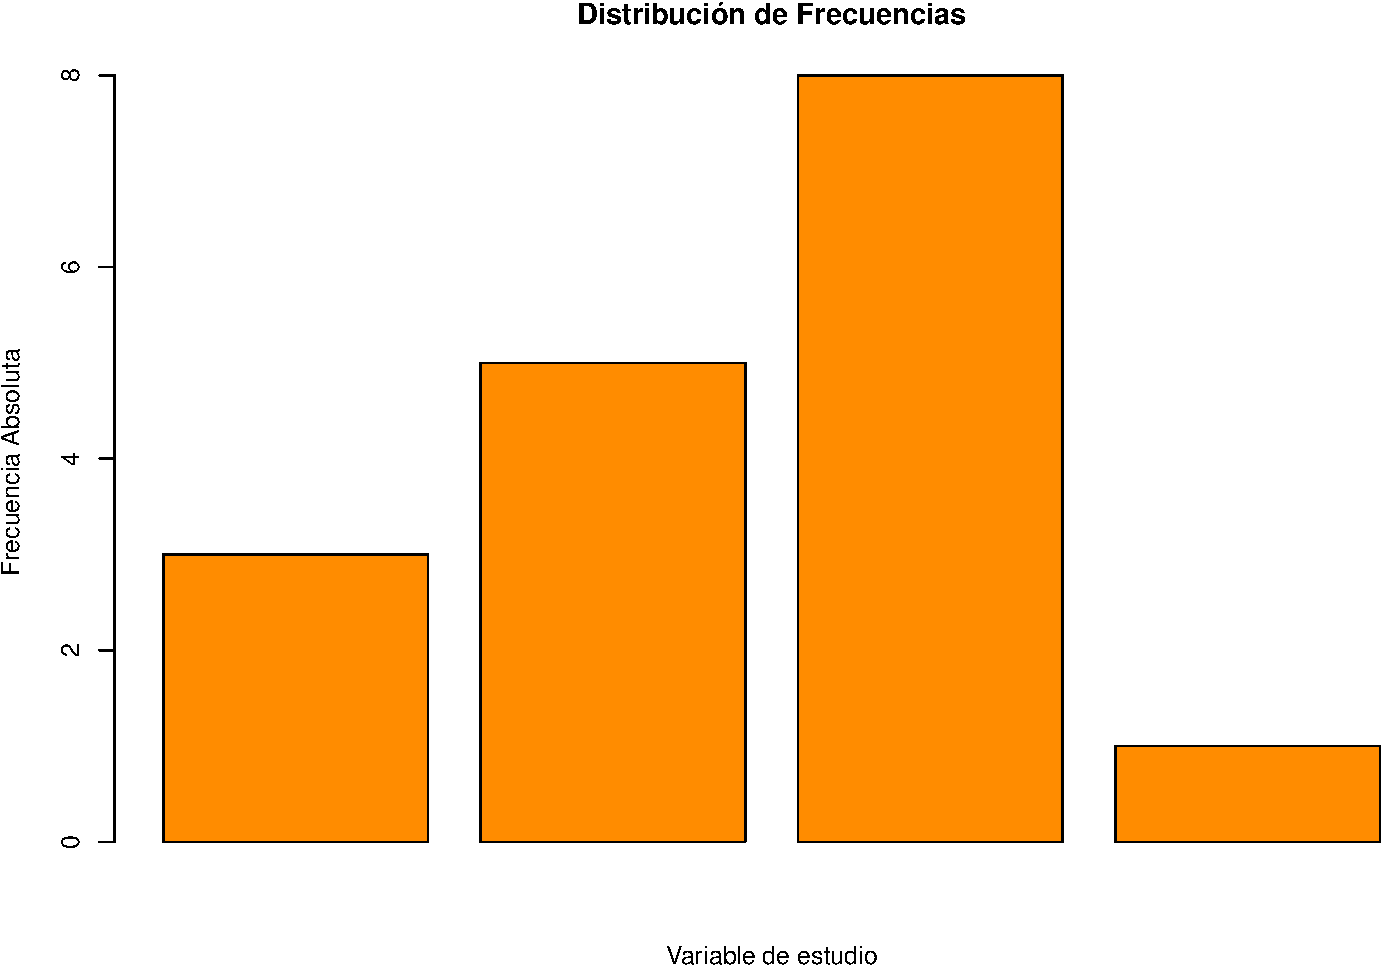
\includegraphics[keepaspectratio]{PlantilaQuartoTallerTFrecSimples_files/figure-beamer/grafico-barras-personalizado-1.pdf}}
\end{frame}

\begin{frame}{Declaración de Autoría}
\phantomsection\label{declaraciuxf3n-de-autoruxeda}
\begin{tcolorbox}[enhanced jigsaw, opacitybacktitle=0.6, toprule=.15mm, opacityback=0, colbacktitle=quarto-callout-note-color!10!white, colback=white, leftrule=.75mm, bottomrule=.15mm, colframe=quarto-callout-note-color-frame, titlerule=0mm, coltitle=black, bottomtitle=1mm, breakable, rightrule=.15mm, toptitle=1mm, title=\textcolor{quarto-callout-note-color}{\faInfo}\hspace{0.5em}{Note}, arc=.35mm, left=2mm]

Yo, {[}Nombre del Estudiante{]}, declaro que el análisis y las
interpretaciones presentadas en este informe son de mi autoría. Entiendo
que el uso de herramientas de IA debe ser declarada y que la
coincidencia exacta de texto con otros compañeros será penalizada con
una considerable baja en la nota y, si hay méritas, según el reglamento
docente.

\end{tcolorbox}
\end{frame}




\end{document}
